\chapter{Analisi e progettazione concettuale}

In questo capitolo verranno analizzati la struttura e lo sviluppo della base di dati su cui si appoggia l'applicazione, useremo un diagramma molto usato nella progettazione, chiamato \textbf{diagramma ER} (Entità-Relazione)

\section{Analisi dei requisiti}

Inizialmente, per la progettazione di una base di dati è necessario raccogliere i requisiti che il database deve soddisfare. Si intende così, l'individuaione dei problemi che l'applicazione deve risolvere oltre alle caratteristiche che dovrà assumente.

I requisiti vengono raccolti in specifiche espresse generalmente in linguaggio naturale e in modo confusionale, per questo l'analisi dei requisiti viene in aiuto chiarendo e organizzando le specifiche. 
\\
I requisiti raccolti duranti la progettazione di Inline sono:\\\\
\textbf{User}
\begin{itemize}
	\item ID, identificativo unico incrementante
	\item Username, Il nome scelto per l'utente
	\item Password, Una parola che rispetti i requisiti scelta dall'utente
	\item RoomAttended, Il numero delle stanze a cui questo utente ha partecipato
	\item Admin, Un campo booleano che denota se l'utente è amministratore
	\item Rating, Un campo che specifica il rating utente
	\item CreatedAt, Campo che specifica la data di creazione
	\item UpdatedAt, Campo che specifica l'ultima modifica del profilo
	\item Varie colonne JSON per la rappresentazione dei social network.
	\item Altre colonne accessorie come 'ResetDigest', 'Invitations', 'ResetSentAt'
\end{itemize}

\textbf{Room}
\begin{itemize}
	\item ID, identificativo unico incrementante
	\item Nome, Il nome scelto per la room
	\item Fifo, Un boolean che descrive la tipologia delle code
	\item MaxParticipants, Un campo integer che contiene il massimo numero di partecipanti
	\item Latitude, Latitudine del luogo in cui si terrà la room
	\item Longitude, Longitudine del luogo in cui si terrà la room
	\item Private, Un boolean che descrive se la room è privata
	\item CreatedAt, Campo che specifica la data di creazione
	\item UpdatedAt, Campo che specifica l'ultima modifica della room
	\item Description, Campo che continene una descrizione della room
	\item Adress, Campo che contiene l'indirizzo in cui si terrà la room
\end{itemize}

\textbf{Prenotazione}
\begin{itemize}
	\item IDUser, Identificativo dell'utente
	\item IDRoom, Identificativo della room
	\item CreatedAt, Campo che specifica la data di creazione della prenotazione
	\item UpdatedAt, Campo che specifica l'ultima modifica della prenotazione
\end{itemize}

\textbf{Mailbox}
\begin{itemize}
	\item IDUser, Identificativo del mittente
	\item IDRoom, Identificativo della room
	\item Body, Il corpo del messaggio
	\item ReceiverType, Il tipo del destinatario
	\item ReceiverId, L'id del destinatario
	\item Una serie di campi per confermare la lettura, modifica e cancellazione del messaggio
\end{itemize}

\section{Diagramma ER}
Nell'ambito della progettazione dei database il modello Entità-Relazione è un modello per la rappresentazione concettuale e grafica dei dati a un alto livello di astrazione.

Il modello ER viene spesso utilizzato nella prima fase della progettazione di una base di dati in cui è necessario tradurre le informazione risultanti dell'analisi di un determinato dominio in uno schema concettuale.

Nell'ambito della progettazione ingegneristice delle basi di dati si distringuono in tre livello indipendenti e consecutivi di progettazione: \textit{Progettazione concettuale, progettazione logica, progettazione fisica.}

I principali costrutti del diagramma sono:
\begin{itemize}
	\item Le entità
	\item Le associazione
	\item Gli attributi
	\item La cardinalità
\end{itemize}

Nella prossima pagina sarà riportato il diagramma entità-relazione di Inline, nel quale si descrive la creazione di una room da parte dell'utente.
Ogni diagramma deve essere accompagnato da una documentazione che lo descrive in tutte le sue componenti. 

Le successive tabelle mostrano ciò che viene chiamato il dizionario dei dati associato al diagramma ER, costituito dalle tabelle dell'entità, delle relazione e degli attributi.

\begin{figure}[H]
	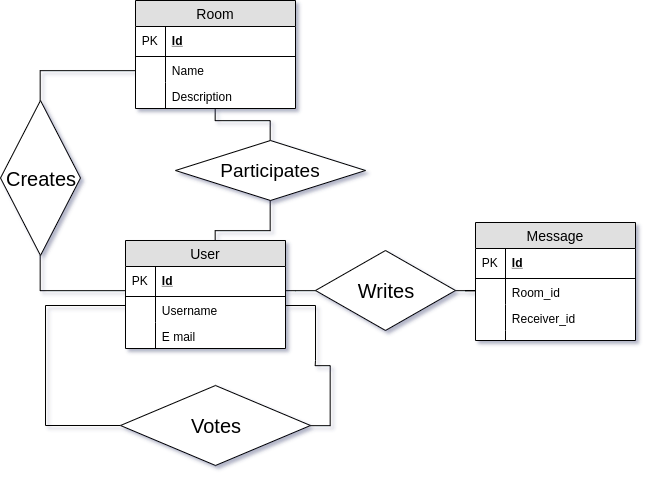
\includegraphics[width=\columnwidth]{./media/ER.png}
	\caption{Diagramma ER}
\end{figure}

\section{Dizionario dei dati: Entità}
Nella prima colonna troviamo le entità, cioè gli elementi cardine dello schema, nonchè tabelle principale nella base di dati dell'applicazione. Nella seconda colonna è presente una descrizione che aiuta a comprendere meglio l'elemento precedente. Nella terza colonna troviamo gli attributi che rappresentano le colonne nel database. Per ultimo, ma non per importanza, troviamo l'identificatore della riga.\newline

\begin{table}[H]
	\centering
	\caption{Tabella delle entità}
	\begin{tabularx}{\textwidth}{l c X}
		\toprule
		Entità & Identificativo & Attributi\\
		\midrule
		\textbf{User} & ID & \textbf{ID}, Username, Email, Password, Admin, Rating, Invitations, Rooms attended \\
		\textbf{Room} & ID & \textbf{ID}, Nome, Descrizione, Fifo, MaxParticipants, Address, Latitude, Longitude, Private, MaxUnjoinTime, TimeFrom, TimeTo, Recurrence, EventId, UserId \\
		\textbf{Message} & ID & \textbf{ID}, RoomId, ReceiverId, NotificationId, IsRead, isDelivered, Trashed, Deleted, MailboxType, deliveryMethod, MessageId \\
		\bottomrule
	\end{tabularx}
\end{table}

\section{Dizionario dei dati: Relazioni}
Le relazioni, rappresentate con dei rombi nel diagramma ER costituiscono i legami che ci sono tra \textit{minimo} due entità. In base al numero di entità coinvolte possiamo definire il grado della relazione.
\begin{table}[H]
	\centering
	\caption{Tabella delle relazioni}
	\begin{tabularx}{\textwidth}{l X c}
		\toprule
		Relazione & Descrizione & Componenti\\
		\midrule
		\textbf{Creates} & Creazione di una room da parte di un utente & User, Room \\
		\textbf{Participates} & Partecipazione di un utente ad una room & User, Room \\
		\textbf{Writes} & Scrittura e pubblicazione di un messaggio da parte di un utente & User, Message\\
		\textbf{Votes} & Votazione di un utente verso un altro utente & User \\
		\bottomrule
	\end{tabularx}
\end{table}

\section{Dizionario dei dati: Attributi}
Attraverso tre tabelle nomineremo tutti gli attributi presenti nello schema ER menzionando il dominio, l'entità.
La prima colonna citerà il nome dell'attributo, sarà in grassetto se è un identificatore, la seconda l'entità alla quale appartiene ed infine, la terza definirà il dominio.

\begin{table}[H]
	\centering
	\caption{Tabella degli attributi user}
	\begin{tabular}{l c r}
		\toprule
		Attributo & Entità & Dominio\\
		\midrule
		\textbf{ID} & User & Integer \\
		Username & User & String \\
		Email & User & String \\
		Password & User & String \\
		Rating & User & Json \\
		Invitations & User & Json\\
		RoomsAttended & User & Integer\\
		Admin & User & Boolean\\
		\bottomrule
	\end{tabular}
\end{table}

\begin{table}[H]
	\centering
	\caption{Tabella degli attributi room}
	\begin{tabular}{l c r}
		\toprule
		Attributo & Entità & Dominio\\
		\midrule
		\textbf{ID} & Room & Integer \\
		Name & Room & String \\
		Description & Room & String \\
		Fifo & Room & Boolean\\
		MaxParticipants & Room & Integer\\
		Address & Room & String\\
		Latitude & Room & Float\\
		Longitude & Room & Float\\
		Private & Room & Boolean\\
		MaxUnjoinTime & Room & Datetime\\
		TimeFrom & Room & Datetime\\
		TimeTo & Room & Datetime\\
		Recurrence & Room & Text\\
		EventId & Room & String\\
		UserId & Room & String\\
		\bottomrule
	\end{tabular}
\end{table}

\begin{table}[H]
	\centering
	\caption{Tabella degli attributi message}
	\begin{tabular}{l c r}
		\toprule
		Attributo & Entità & Dominio\\
		\midrule
		\textbf{ID} & Room & Integer \\
		RoomId & Message & Integer \\
		UserId & Message & Integer\\
		ReceiverType & Message & String\\
		ReceiverId & Message & Integer\\
		NotificationId & Message & Integer\\
		IsRead & Message & Boolean\\
		IsDelivered & Message & Boolean\\
		Trashed & Message & Boolean\\
		MailboxType & Message & String\\
		DeliveryMethod & Message & String\\
		MessageId & Message & String\\
		\bottomrule
	\end{tabular}
\end{table}

\section{Dizionario dei dati: vincoli di cardinalità}
Un vincolo di cardinalità associa ad un ruolo \textbf{U} corrispondente ad un entità \textbf{E} in una relazione \textbf{R}, ed impone un limite minimo e massimo di istanze della relazione a cui può partecipare ogni istanza dell'entità \textbf{E} nel ruolo \textbf{U}. In inline abbiamo tutti i tipi di vincoli del tipo 0..* 